\chapter{Mesures, dénominateurs et sensibilité}\label{ch:mesures}

Les fréquences décrivent les documents conservés et les règles de leur traitement. Elles ne deviennent des estimations de la société antique qu’au prix d’hypothèses supplémentaires sur la sélection, la conservation et la publication des textes. Le corpus n’ayant pas été tiré au hasard, aucune marge d’erreur calculée sous un modèle binomial ne résume ces incertitudes documentaires. Ce chapitre présente les principales mesures du volume, les dénominateurs qui les fondent et leur sensibilité aux choix de définition.

\section{Les dénominateurs}

Toutes les mesures du formulaire, du vocabulaire religieux, des âges et des signes sont rapportées à l’ensemble C (\st{nC} textes funéraires ; chapitre~\ref{ch:corpus}). Trois choix de définition commandent cet effectif :

\begin{itemize}
\item \emph{les doublons} : les trois paires de notices qui transmettent le même monument (106/120, 282/288 et 329/336) sont fusionnées, et le fragment 394 est joint au 393 ; chaque monument n’est compté qu’une fois ;
\item \emph{la période} : le \nnum{98}, daté de 461 ou 482, est exclu ;
\item \emph{le genre} : les sept actes d’achat sans commémoration et l’inscription architecturale de la colonne de Saint-Paul sont exclus ; les sept textes mixtes, dont le \nnum{406}, sont inclus.
\end{itemize}

Le dénominateur de la version précédente (468 textes) comptait séparément deux des monuments dédoublés (\nnums{106} et 282) et le fragment 394, incluait le \nnum{98} et excluait le \nnum{406}. Les mesures qui en dépendent ont toutes été recalculées.

\section{Principales mesures et intervalles}

Le tableau~\ref{tab:mesures} donne les principales mesures selon trois dénominateurs : l’ensemble C ; les textes dont l’année repose sur une formule consulaire lue ou transmise par l’EDB (\st{nCdirect} textes) ; les textes dont la lecture est concordante entre l’EDCS et l’EDB (\st{nCstab} textes, « lectures stabilisées »).

% généré par scripts/04_generated.py
\begin{longtable}{@{}p{0.27\linewidth} p{0.27\linewidth} r r r l@{}}\caption{Principales mesures selon trois dénominateurs. Les intervalles de Wilson (95~\%) sont des résumés binomiaux conditionnels, non des marges d’erreur sur la population antique.}\label{tab:mesures}\\
\toprule Mesure & Ensemble & n & k & \% & IC 95 \%\\\midrule\endfirsthead\toprule Mesure & Ensemble & n & k & \% & IC 95 \%\\\midrule\endhead\bottomrule\endfoot
in pace (attestée) & C & 465 & 193 & 41,5 & 37,1–46,0 \\
in pace (attestée) & C, datation directe ou transmise & 457 & 193 & 42,2 & 37,8–46,8 \\
in pace (attestée) & C, lecture concordante EDCS/EDB & 281 & 137 & 48,8 & 43,0–54,6 \\
in pace (en toutes lettres) & C & 465 & 129 & 27,7 & 23,9–32,0 \\
in pace (en toutes lettres) & C, datation directe ou transmise & 457 & 129 & 28,2 & 24,3–32,5 \\
in pace (en toutes lettres) & C, lecture concordante EDCS/EDB & 281 & 100 & 35,6 & 30,2–41,3 \\
Profil religieux large (niv. 1–2) & C & 465 & 13 & 2,8 & 1,6–4,7 \\
Profil religieux large (niv. 1–2) & C, datation directe ou transmise & 457 & 13 & 2,8 & 1,7–4,8 \\
Profil religieux large (niv. 1–2) & C, lecture concordante EDCS/EDB & 281 & 9 & 3,2 & 1,7–6,0 \\
Profil religieux strict & C & 465 & 8 & 1,7 & 0,9–3,4 \\
Profil religieux strict & C, datation directe ou transmise & 457 & 8 & 1,8 & 0,9–3,4 \\
Profil religieux strict & C, lecture concordante EDCS/EDB & 281 & 4 & 1,4 & 0,6–3,6 \\
Chrisme ou croix (EDB) & C & 465 & 67 & 14,4 & 11,5–17,9 \\
Chrisme ou croix (EDB) & C, datation directe ou transmise & 457 & 65 & 14,2 & 11,3–17,7 \\
Chrisme ou croix (EDB) & C, lecture concordante EDCS/EDB & 281 & 52 & 18,5 & 14,4–23,5 \\
Texte grec ou bilingue & C & 465 & 7 & 1,5 & 0,7–3,1 \\
Texte grec ou bilingue & C, datation directe ou transmise & 457 & 6 & 1,3 & 0,6–2,8 \\
Texte grec ou bilingue & C, lecture concordante EDCS/EDB & 281 & 4 & 1,4 & 0,6–3,6 \\
Âge indiqué & C & 465 & 206 & 44,3 & 39,9–48,8 \\
Âge indiqué & C, datation directe ou transmise & 457 & 205 & 44,9 & 40,4–49,4 \\
Âge indiqué & C, lecture concordante EDCS/EDB & 281 & 152 & 54,1 & 48,2–59,8 \\
Plus de la moitié des lettres restituées & C & 465 & 101 & 21,7 & 18,2–25,7 \\
Plus de la moitié des lettres restituées & C, datation directe ou transmise & 457 & 101 & 22,1 & 18,5–26,1 \\
Plus de la moitié des lettres restituées & C, lecture concordante EDCS/EDB & 281 & 32 & 11,4 & 8,2–15,6 \\
\end{longtable}


Les intervalles de Wilson ont un sens sous un modèle binomial conditionnel. Ils ne couvrent ni les lacunes, ni les doublons non reconnus, ni les erreurs de lecture, ni les choix d’inclusion, et ne sont pas des intervalles de confiance sur l’ensemble des chrétiens de Rome. Ils indiquent seulement l’ordre de grandeur de la variation que produirait le hasard sur des effectifs de cette taille.

\section{Sensibilité aux choix d’inclusion}

La formule \emph{in pace} sert de mesure témoin.

\begin{itemize}
\item Dans l’ensemble C : \st{sensC}.
\item Sans le \nnum{406}, dont la qualification de texte funéraire peut se discuter : \st{sens406}.
\item Sur les seuls textes à datation directe ou transmise : \st{sensDirect}.
\item Sur les seules lectures stabilisées entre les deux bases : \st{sensStab}.
\end{itemize}

Les trois premiers choix ne déplacent la proportion que de quelques dixièmes de point. Le quatrième la déplace de sept points. Ce n’est pas un effet de la formule elle-même : les textes dont la lecture concorde entre les deux bases sont, en moyenne, mieux conservés (11~\% seulement ont plus de la moitié de leurs lettres restituées, contre 22~\% dans l’ensemble C) et plus longs, donc plus susceptibles de contenir chaque élément du formulaire. La même hausse s’observe pour l’âge (54~\% contre 44~\%) et pour les signes (18~\% contre 14~\%). La sélection des lectures stabilisées n’est donc pas un sous-ensemble neutre : elle favorise les textes complets.

\section{Sensibilité au traitement des restitutions}

Le traitement des restitutions a un effet plus important que les choix d’inclusion. Pour \emph{in pace}, la proportion passe de \st{ip_pct}~\% (restitutions comprises) à 31,6~\% (attestations sans restitution) et à \st{ip_ecrit_pct}~\% (formule écrite en toutes lettres, sans abréviation ni correction). Pour le vocabulaire religieux, la proportion passe de 3,9~\% (restitutions comprises) à 2,8, 2,4 ou 1,7~\% selon les trois profils (chapitre~\ref{ch:typologie}). Pour les comparaisons chronologiques, la part des lettres restituées augmente avec le temps (ratio moyen de 0,26 en 340–359, 0,29 en 390–403), ce qui suffit à produire un recul apparent des éléments comptés sans restitution (chapitre~\ref{ch:formulaire}).

Ces écarts sont la principale incertitude du volume. Ils ne peuvent être réduits que par un retour aux éditions imprimées et aux photographies.

\section{La part restituée des textes}

\begin{figure}[tbp]\centering
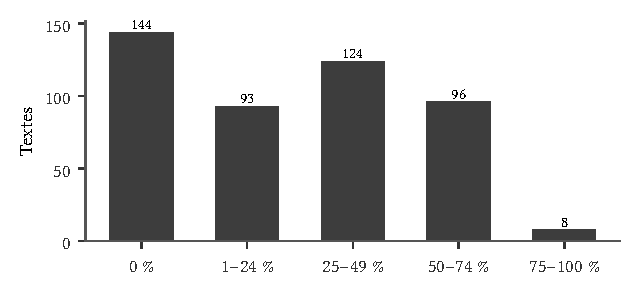
\includegraphics[width=0.8\linewidth]{figures/fig_restitution.pdf}
\caption{Part des lettres restituées par texte (ensemble C).}\label{fig:restitution}
\end{figure}

La figure~\ref{fig:restitution} donne la distribution de la part des lettres restituées. \st{nZeroRest} textes de l’ensemble C ne comportent aucune lettre restituée ; \st{nPlusMoitie} en ont plus de la moitié. Cette distribution rappelle qu’une grande partie du corpus est fragmentaire, et que toute mesure fondée sur le texte « avec restitutions » mesure, pour une part, le travail des éditeurs.
